% $Id$
% Author: Daniel Bosk <daniel.bosk@miun.se>
\documentclass{beamer} % [handout]
\usepackage[utf8]{inputenc}
\usepackage[T1]{fontenc}
\usepackage[english,swedish]{babel}
\usepackage{url}
\usepackage{varioref,prettyref}
\usepackage{graphicx}
\usepackage[today,nofancy]{svninfo}
\usepackage{natbib}
\usepackage{listings}
\usepackage{color}
\usepackage{subfig}
\usepackage[binary,amssymb]{SIunits}
\usepackage[varioref,prettyref,listings]{miunmisc}
\setcitestyle{numbers,square}
\bibliographystyle{swealpha}

% default style for listings is code and default language is TeX
\lstset{style=code,language=tex}

\svnInfo $Id$

\mode<presentation>
{
	\usetheme{Frankfurt}
	\setbeamercovered{transparent}
  %\usecolortheme{default}
	\usecolortheme{seagull}
}
\setbeamertemplate{footline}{\insertframenumber}

\title{%
	\LaTeX
}
\author{Daniel Bosk}
\institute[MIUN ITM]{%
	%Division of Information and Communication Systems (ICS),\\
	%Department of Information Technology and Media (ITM),\\
	%Mid Sweden University, Sundsvall.
	%
	%Avdelningen för informations- och kommunikationssytem (IKS),\\
	Institutionen för informationsteknologi och medier (ITM),\\
	Mittuniversitetet, Sundsvall.
}
\date{\svnId}

% use the logotype in the slides
\pgfdeclareimage[height=0.65cm]{university-logo}{MU_logotyp_int_CMYK.pdf}
\logo{\pgfuseimage{university-logo}}

\AtBeginSection[]{%
	% show table of contents at beginning of every section
	\begin{frame}<beamer>{Översikt}
		\tableofcontents[currentsection]
	\end{frame}
}

\begin{document}

\begin{frame}
  \titlepage
\end{frame}
\begin{frame}{Översikt}
	\tableofcontents%[pausesections]
\end{frame}

\section{Historia}

\subsection{Metafont, \TeX{} och \LaTeX{}}
\begin{frame}{Metafont, \TeX{} och \LaTeX{}}
	\begin{itemize}
		\item \TeX{} skapades av Donald E. Knuth, Standford University, i slutet av 
			1970-talet.
			\begin{itemize}
				\item Ville att \emph{The Art of Computer Programming} 
					\citep{Knuth1997tao} skulle typsättas vackrare.
			\end{itemize}
		\item \LaTeX{} skapades av Leslie Lamport 1985.
			\begin{itemize}
				\item Skapat för att enkelt typsätta dokument av olika slag.
				\item Används flitigt inom akademin.
			\end{itemize}
	\end{itemize}
\end{frame}

\subsection{Några exempel}
\begin{frame}{Några exempel}{The \TeX{} Showcase}
	Några exempel hämtade från \emph{The \TeX{} Showcase} \citep{TUG2012tsc}:
	\begin{figure}
		\subfloat[Kartor.]{%
			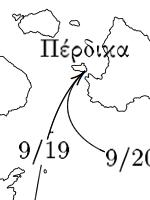
\includegraphics[width=0.2\linewidth]{maps.jpg}
		}
		\hfill
		\subfloat[Musik och noter.]{%
			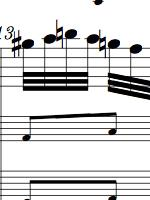
\includegraphics[width=0.2\linewidth]{music.jpg}
		}
		\hfill
		\subfloat[Cirkulär marginal.]{%
			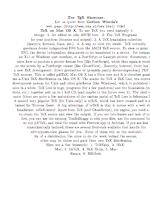
\includegraphics[width=0.2\linewidth]{circular_margin.jpg}
		}
		\hfill
		\subfloat[Tolkiens tengwar.]{%
			
\includegraphics[width=0.2\linewidth]{tengwar.jpg}
		}
	\end{figure}
\end{frame}


\section[Dokumentstruktur]{Övergripande dokumentstruktur}

\subsection{Preamble}
\begin{frame}[fragile]{Preamble}
	\begin{lstlisting}
\documentclass[a4paper]{article}
\usepackage[utf8]{inputenc}
\usepackage[T1]{fontenc}
\usepackage[english,swedish]{babel}

\author{Daniel Bosk}
\title{Testdokument}
\date{\today}
	\end{lstlisting}
\end{frame}

\subsection{Textinnehållet}
\begin{frame}[fragile]{Textinnehållet}
	\begin{lstlisting}
\begin{document}
	\maketitle
	\tableofcontents

	\dots
\end{document}
	\end{lstlisting}
\end{frame}


\section[Innehåll]{Dokumentets innehåll}

\subsection{Paragrafer och avsnitt}
\begin{frame}{Paragrafer}
	\begin{itemize}
		\item Skrivs som vanlig text.
		\item Olika paragrafer separeras med en blankrad eller kommandot 
			\texttt{\textbackslash par}.
	\end{itemize}
\end{frame}
\begin{frame}{Avsnitt}
	Finns olika typer av avsnitt beroende på vilken dokumentklass som används.
	\begin{description}
		\item[chapter] Betecknar kapitel.
			Finns i klasser som avser större dokument, exempelvis book, report, 
			miunthes.
		\item[section] Betecknar ett avsnitt.
			Finns i alla klasser.
		\item[subsection] Betecknar ett delavsnitt.
			Finns i alla klasser.
		\item[subsubsection] Betecknar den minsta typen av avsnitt som bör 
			användas.
			Finns i de flesta klasser.
	\end{description}
	Dessa används på följande vis:
	\begin{center}
		\texttt{\textbackslash section[Short title]\{Long title\}}
	\end{center}
\end{frame}

\subsection{Referenser}
\begin{frame}[fragile]{Referenser}
	\begin{lstlisting}
...
\usepackage{natbib}
...
Enligt Knuth \cite{Knuth1997tao} finns ingen algoritm för att lösa problemet.
...
\bibliography{literature}
	\end{lstlisting}
	Ger resultatet:
	\begin{quote}
		Enligt Knuth \cite{Knuth1997tao} finns ingen algoritm för att lösa 
		problemet.
	\end{quote}
\end{frame}
\begin{frame}[fragile]{Bib\TeX}{literature.bib}
	\lstinputlisting[firstline=73,lastline=90]{../../literature.bib}
\end{frame}

\subsection{Matematik}
\begin{frame}[fragile]{Matematik}
	\begin{lstlisting}
		Vi har summan \( \sum_{i=1}^n i = \frac{n (n + 1)}{2} \).
		Men sedan har vi även summan \[ \sum_{i=1}^n i = \frac{n (n + 1)}{2} \].
	\end{lstlisting}
	Ger resultatet:
	\begin{quote}
		Vi har summan \( \sum_{i=1}^n i = \frac{n (n + 1)}{2} \).
		Men sedan har vi även summan \[ \sum_{i=1}^n i = \frac{n (n + 1)}{2} \].
	\end{quote}
\end{frame}
\begin{frame}[fragile]{Matematik}
	\begin{lstlisting}
\[ f(a) = \left\{
  \begin{array}{ll}
    y & \text{om } a=x \\
    x & \text{om } a=y
  \end{array}
  \right\} = f^{-1}(a), \]
  \end{lstlisting}
	Detta ger resultatet:
	\begin{quote}
\[ f(a) = \left\{
	\begin{array}{ll}
		y & \text{om } a=x \\
		x & \text{om } a=y
	\end{array}
	\right\} = f^{-1}(a), \]
	\end{quote}
\end{frame}
\begin{frame}{\TeX{} math mode}
	\begin{itemize}
		\item I en del kod kan man stöta på att matematiken avgränsas med 
			dollartecken (\$), detta är \TeX-motsvarigheten till 
			\texttt{\textbackslash (} och \texttt{\textbackslash )}.
		\item På samma sätt dubbla dollartecken (\$\$) för \texttt{\textbackslash 
			[} och \texttt{\textbackslash ]}.
	\end{itemize}
\end{frame}

\subsection{Figurer och tabeller}
\begin{frame}[fragile]{Figurer}
	\begin{lstlisting}
\usepackage{graphicx}
...
\begin{figure}
  \centering
  
\includegraphics[width=0.2\linewidth]{tengwar.jpg}
  \caption{En bild föreställande J. R. R. Tolkiens tengwar.}
  \label{fig:bild}
\end{figure}
	\end{lstlisting}
\end{frame}
\begin{frame}{Figurer}{Den resulterande figuren}
	\begin{figure}
		\centering
		
\includegraphics[width=0.2\linewidth]{tengwar.jpg}
		\caption{En bild föreställande J. R. R. Tolkiens tengwar.}
		\label{fig:bild}
	\end{figure}
\end{frame}
\begin{frame}[fragile,allowframebreaks]{Tabeller}
	\begin{lstlisting}
\begin{table}
  \centering
  \begin{tabular}{r|cccccccccc}
    \hline\hline
    \(\alpha\) & a & b & c & d & e & f & g & h & i & j \\
    \(P_E(\alpha)\) & 8.2  & 1.5 & 2.8 & 4.3 & 12.7 & 2.2 & 2.0 & 6.1 & 7.0 & 0.2 \\
    \(P_S(\alpha)\) & 9.3  & 1.3 & 1.3 & 4.5 & 9.9 & 2.0 & 3.3 & 2.1 & 5.1 & 0.7 \\
    \hline\hline
  \end{tabular}
  \caption{Tabell av sannolikhetsfunktionen för bokstäver i det engelska och det svenska språket, \(P_E\) respektive \(P_S\), angiven i procent med en decimals noggrannhet.}
  \label{tbl:SannolikhetstabellSpråk}
\end{table}
	\end{lstlisting}
\end{frame}
\begin{frame}{Tabeller}{Den resulterande tabellen}
	\begin{table}
		\centering
		\begin{tabular}{r|cccccccccc}
			\hline\hline
			\(\alpha\) & a & b & c & d & e & f & g & h & i & j \\
			\(P_E(\alpha)\) & 8.2  & 1.5 & 2.8 & 4.3 & 12.7 & 2.2 & 2.0 & 6.1 & 7.0 & 0.2 \\
			\(P_S(\alpha)\) & 9.3  & 1.3 & 1.3 & 4.5 & 9.9 & 2.0 & 3.3 & 2.1 & 5.1 & 0.7 \\
			\hline\hline
		\end{tabular}
		\caption{Tabell av sannolikhetsfunktionen för bokstäver i det engelska och 
		det svenska språket, \(P_E\) respektive \(P_S\), angiven i procent med en 
		decimals noggrannhet.}
		\label{tbl:SannolikhetstabellSpråk}
	\end{table}
\end{frame}

\subsection{Cross-referencing}
\begin{frame}[fragile]{Cross-referencing}
	\begin{lstlisting}
För att förstå denna text bör du se tabell \ref{tbl:SannolikhetstabellSpråk}.
	\end{lstlisting}
	\begin{lstlisting}
...
\usepackage[swedish]{babel}
\usepackage{prettyref}
\usepackage[prettyref]{miunmisc}
...
För att förstå denna text bör du se \prettyref{tbl:SannolikhetstabellSpråk}.
	\end{lstlisting}
\end{frame}


\section[Klasser och paket]{Användbara klasser och paket}

\subsection{miunthes}
\begin{frame}[fragile,allowframebreaks]{miunthes}
	\lstinputlisting{thesis.tex}
	\lstinputlisting[lastline=5]{theory.tex}
\end{frame}

\subsection[Standardklasser och paket]{Några standardklasser och paket}
\begin{frame}{Några standardklasser och paket}
	\begin{description}
		\item[SIunits] Används för att korrekt typsätta enheter.
		\item[natbib] Används för att förenkla referenshantering.
			Får exempelvis kommandot \texttt{\textbackslash citet}.
		\item[listings] Används för att lista kod, likt i dessa slides.
	\end{description}
\end{frame}
\begin{frame}[fragile]{SIunits}
	\begin{lstlisting}
...
\usepackage[binary]{SIunits}
...
En linjal i standardutförande är \unit{30}{\centi\metre}, medan 
överföringshastigheten är \unit{1}{\giga\bit\per\second}.
	\end{lstlisting}
	Ger resultatet:
	\begin{quote}
		En linjal i standardutförande är \unit{30}{\centi\metre}, medan 
		överföringshastigheten är \unit{1}{\giga\bit\per\second}.
	\end{quote}
\end{frame}

\subsection{miunmisc}
\begin{frame}[fragile]{miunmisc}
	\begin{lstlisting}
\usepackage{natbib}
\usepackage{listings}
\usepackage{prettyref}
\usepackage{varioref}
\usepackage[natbib,listings,varioref,prettyref]{miunmisc}
	\end{lstlisting}
\end{frame}

\subsection{beamer}
\begin{frame}[allowframebreaks]{beamer}
	\lstinputlisting{latex.tex}
\end{frame}


%%%%%%%%%%%%%%%%%%%%%%

\begin{frame}{Referenser}
	\bibliography{../../literature}
\end{frame}

\end{document}

